\chapter{Application}
\label{chapter:application}


\section{Use cases}
\label{section:useCases}

Before diving into the application architecture and implementation details, let us first describe the use cases to get a complete overview of the functionality the app has to provide (See Fig. \ref{useCase}). The first and the most important use case is registering documents into the system. This would include automatically generating a registration number for each document. It is an important part of automating the current process, in which for registering a new document, the employee has to contact the registry administrator and ask for an available registration number. For the registration to be complete, the user has to specify a destination for the document. In most cases, the document would be internal, meaning that the destination would be other employees of the institution. In this case, the document is sent to the specified recipients, which receive an email notification and could then view the received documents in their account. However, some documents could have an external destination, like another institution or organization. In this case, the destination is specified so the document could be easily tracked in the future. Analogically, the issuer could specify an external source of the document, if it has one.

The user could upload an electronic version of the document, either immediately after the registration, or in any point of time in the future. Additionally, the upload feature is available for all recipients of a document.

The logic behind the document management process relies mainly on two actions: resolving and archiving a document. Basically, when a user receives a document, it means that he or she is expected to perform an action related to it. It could be an action as trivial as aknowledging that the document was received, or something more complex like reading and approving the document, uploading an edited version of the document or sending it further to other users. Regardless of this, the \textbf{resolve} action is meant to finalize the interaction between a user and a document.
\begin{figure}[H]
    \centering
    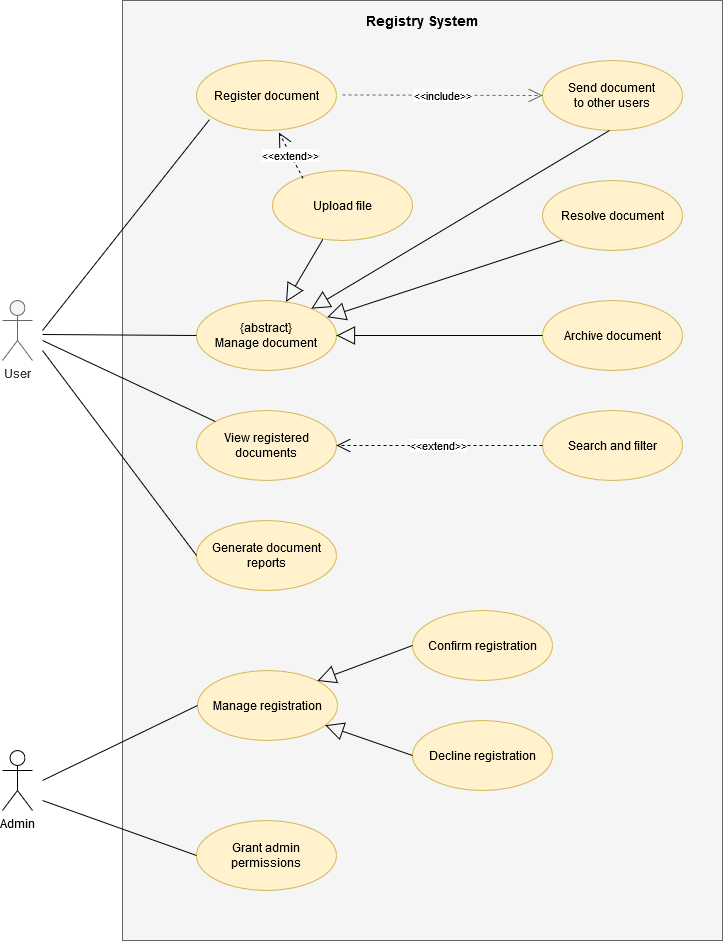
\includegraphics[width=5in]{images/useCase}
    \caption{Registry System Use Cases}
    \label{useCase}
\end{figure}
In simpler terms, marking a document as resolved is telling its issuer that all necessary actions from the receiver were taken.

The \textbf{archive} action, on the other hand, is meant to complete the document lifecycle and can only be performed by the document issuer. After a document is marked as archived, it could no longer get resolved or sent to other users. Resolving and archiving a document are closely related actions. After all, it seems rather logical that the user should only archive a document after it has been resolved by its receiver. However, the logic gets more complicated in case multiple receivers are specified. It could be that all of them have to take different actions on the document. It could also be that getting the document resolved by only one of them would be sufficient, like if, for example, they are employees of the same department. In this case, getting a document resolved by a receiver is not a required constraint for the document to get archived. Similarily, when a document is resolved, it does not necessarily imply that it should immediately get archived. That is why we have not constrained the ability to archive a document based on whether it was resolved, but rather let the issuer do it the document when he or she deems it necessary.






\section{Implementation}
\label{section:implementation}

\section{Architecture}
\label{section:architecture}

